

\chapter{Einleitung}
\section{Vorwort}
Es soll ein Beispiel-Client für den RFU6xx implementiert werden. Dieser Client baut eine Verbindung mit dem RFU6xx auf, indem es das \ac{opcua}-Protokoll und die Programmiersprache node.js nutzt.

\ac{opcua} ist ein offener, plattformunabhängiger Kommunikationsstandard, der für die Übertragung von Daten in industriellen Automatisierungssystemen verwendet wird. Es ermöglicht die Übertragung von Daten, Befehlen und Alarmen zwischen Geräten und Anwendungen in Echtzeit und sorgt für eine sichere und zuverlässige Übertragung.\\

Node.js ist eine serverseitige JavaScript-Laufzeitumgebung, die es Entwicklern ermöglicht, Netzwerkanwendungen zu erstellen. Es ist eine Open-Source-Plattform, die auf Google Chrome's JavaScript-Engine V8 aufbaut und eine Event-gesteuerte, asynchrone Programmierung unterstützt.\\
Im Kontext des RFU6xx-Clients wird node.js verwendet, um eine Verbindung mit dem RFU6xx-Sensor herzustellen, indem es das \ac{opcua}-Protokoll nutzt. Durch die Verwendung von node.js kann eine Anwendung erstellt werden, die Daten von dem Sensor in Echtzeit abruft und verarbeitet.\\

Das \ac{opcua}-Protokoll wird verwendet, um die Verbindung zwischen dem RFU6xx-Client und dem Sensor herzustellen und die Übertragung von Daten, Befehlen und Alarmen sicherzustellen. Mit \ac{opcua} kann eine einheitliche Architektur für die Datenkommunikation bereitgestellt werden, die eine einfache Integration in andere Systeme ermöglicht.\\

In dieser Arbeit wird der RFU6xx-Client unter node.js Implementiert. Der RFU6xx-Client soll die grundlegenden Funktionen des Sensors aufrufen.\\

Der \ac{rfid} RFU6xx ist ein \ac{rfid} Reader, dessen grundlegende Funktion darin besteht, Daten von \ac{rfid}-Tags oder -Transpondern zu lesen und zu übertragen.\\

Ein \ac{rfid}-System besteht aus einem \ac{rfid}-Reader, einer Antenne und \ac{rfid}-Tags oder -Transpondern. Der Reader sendet ein Signal über die Antenne, welches von dem Tag empfangen wird. Der Tag reagiert auf das Signal und sendet seine Daten an den Reader zurück, welcher diese dann verarbeitet.\\

Der RFU63x / RFU630 ist ein industrieller \ac{rfid}-Reader, der für den Einsatz in automatisierten Systemen und Prozessen konzipiert wurde. Er ist in der Lage, Daten in Echtzeit von \ac{rfid}-Tags und -Transpondern zu lesen und zu übertragen. Mit dem RFU63x / RFU630 können Daten schnell und zuverlässig gesammelt werden, was zu einer effizienteren Überwachung und Kontrolle von Prozessen und Lieferkettensystemen führt.\\

So kann eine Verbindung mit dem RFU6xx unter einer weiteren Programmiersprache aufgebaut werden, andererseits nutzte Volkswagen den RFU6xx auch unter node-opcua.

Bei Volkswagen treten bestimmte Fehler auf, die nur auftreten, wenn man den Sensor unter node-opcua verwendet. Um die Ursache dieses Fehlers zu finden, muss zunächst die Verbindung unter node-opcua aufgebaut werden.
Bisher gibt es RFU6xx-Clients, die in Python, C\# und C geschrieben wurden und unter dem \ac{opcua}-Protokoll laufen. 
Der Python Client wurde zu erst von \BetreuerFirma geschrieben nach seinem Abbild wurden die anderen Clients geschrieben. \\
Es gibt noch keinen Sick internen \ac{opcua}-Client der mit node.js geschrieben wurde. Der node.js \ac{opcua}-Client wird mit Hilfe der Biblioteken von node-opcua \cite{GitHub.06.02.2023} implementiert.\\

\section{Projektumfeld}
Zunächst werden das Unternehmen und die Abteilung, in der das Projekt umgesetzt wird,
kurz vorgestellt. Ziel ist es, einen Überblick über die Ausgangssituation der vorliegenden
Arbeit zu geben.

\iffalse
\subsection{SICK AG}

Sick AG ist ein weltweit tätiger Anbieter von Sensoren und Sensorlösungen für industrielle Anwendungen. Das Unternehmen wurde 1946 gegründet und hat seitdem eine expansiven Entwicklung durchgemacht. Sick AG konzentriert sich auf die Bereitstellung innovativer Produkte und Dienstleistungen, die dazu beitragen, die Sicherheit und Effizienz industrieller Prozesse zu verbessern.\\

Eines der Hauptprodukte von Sick AG sind die Sicherheitssensoren. Diese Sensoren werden entwickelt, um potenzielle Gefahren in Arbeitsumgebungen zu erkennen und automatisch dafür zu sorgen, dass Maschinen stillgelegt werden, um Verletzungen von Arbeitnehmern zu vermeiden. Sie finden häufig Anwendung in Bereichen wie automatisierten Maschinen, Materialbewegungssystemen und Montagelinien.\\

Zusätzlich zu den Sicherheitssensoren bietet Sick AG auch eine Reihe von Sensoren für Prozessautomatisierung an. Diese Sensoren dienen zur Überwachung verschiedener Parameter wie Temperatur, Druck und Flüssigkeitspegel in industriellen Prozessen. Sie spielen eine entscheidende Rolle bei der Aufrechterhaltung der Effizienz und Zuverlässigkeit dieser Prozesse.\\

Sick AG legt großen Wert auf Forschung und Entwicklung, um den Bedürfnissen seiner Kunden gerecht zu werden. Das Unternehmen investiert kontinuierlich in Forschung und Entwicklung, um neue und verbesserte Sensor-Technologien zu entwickeln und bestehende Produkte zu optimieren. Diese Bemühungen haben bereits zu einer Vielzahl an Patenten und Auszeichnungen geführt und Sick AG als einen bedeutenden Akteur in der Sensor-Branche etabliert.\\

%Abschließend ist Sick AG ein Unternehmen, das sich darauf konzentriert, industrielle Prozesse durch die Bereitstellung innovativer Sensorlösungen zu verbessern. Durch seinen Fokus auf Sicherheit, Effizienz und Forschung und Entwicklung ist das Unternehmen gut aufgestellt, um weiterhin erfolgreich zu sein.\\
\begin{figure}[htp]
    \centering
    
\includegraphics[width=(\textwidth/2)]{Bild/SICK_Headquarter.jpg}
    \caption{Hauptstandort der SICK AG\cite{.08.10.2016}}
    \label{fig:Hauptstandort der SICK AG}
\end{figure}
\fi
\subsection{Autonomous Perception}

Das Sick Business Cluster Autonomous Perception ist ein Teilbereich von Sick AG, der sich auf die Entwicklung von autonomen Wahrnehmungslösungen für den Einsatz in der Industrie konzentriert. Diese Lösungen ermöglichen es maschinellen Systemen, ihre Umgebung aktiv zu erkennen und auszuwerten, um dadurch sicherer und effizienter zu arbeiten.\\

Das Sick Business Cluster Autonomous Perception bietet eine Vielzahl von Produkten und Dienstleistungen, einschließlich 3D-Kameras, LIDAR-Sensoren und Software-Tools für die Datenanalyse. Diese Technologien ermöglichen es maschinellen Systemen, ihre Umgebung zu verstehen und Entscheidungen auf der Grundlage dieser Informationen zu treffen.\\

Einer der Hauptvorteile des Sick Business Cluster Autonomous Perception ist, dass es die Sicherheit und Effizienz in industriellen Prozessen erhöht. Durch die Fähigkeit, ihre Umgebung zu erkennen und auszuwerten, können maschinelle Systeme besser auf potenzielle Gefahren reagieren und vermeiden, dass sie Unfälle verursachen. Zusätzlich ermöglicht die Fähigkeit zur Datenanalyse, dass maschinelle Systeme ihre Leistung optimieren und ineffiziente Prozesse identifizieren und verbessern können.\\

\begin{figure}[htp]
    \centering
    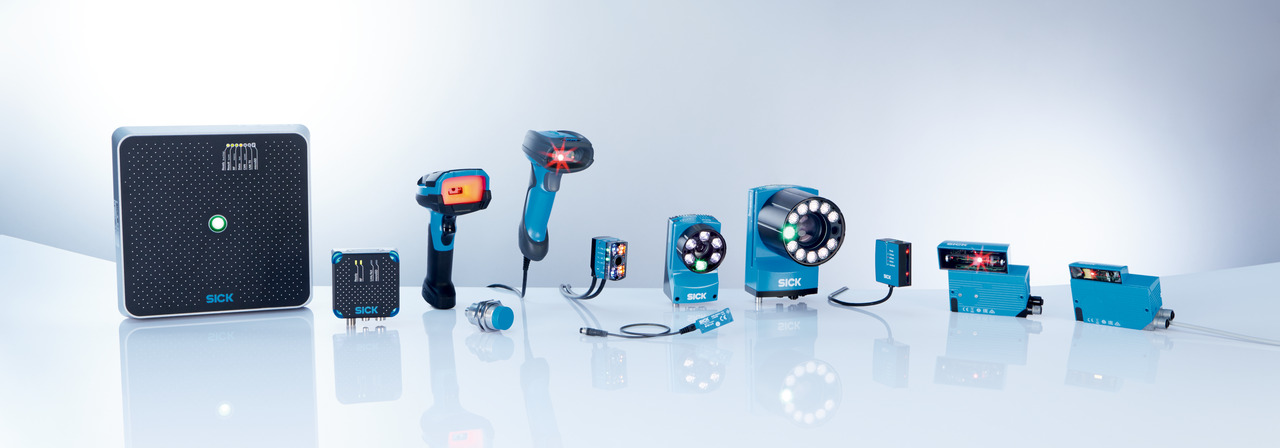
\includegraphics[width=(\textwidth)]{Bild/Identification solutions.jpg}
    \caption{Autonomous Perception\cite{.17.08.2021}}
    \label{fig:Autonomous Perception}
\end{figure}


\section{Problemstellung}
Die Problemstellung bei der Erstellung eines RFU-Client mit node-opcua liegt darin, eine effiziente und stabile Verbindung mit einem \ac{opcua}-Server herzustellen, um Daten auszutauschen und Anfragen zu stellen. 
Dies erfordert ein Verständnis der \ac{opcua}-Kommunikationsprotokolle und der Verwendung der node-opcua-Bibliothek, um die gewünschten Funktionalitäten zu implementieren. Mögliche Herausforderungen können darin bestehen, Fehlerbehandlungen zu implementieren, die Leistung zu optimieren und sicherzustellen, dass die Anwendung den Anforderungen des Benutzers entspricht.
\section{Ziel der Arbeit}
Das Ziel dieser Arbeit ist es, einen \ac{opcua}-Client in Node.js zu entwickeln, der in der Lage ist, sich mit dem Server des SICK RFUs zu verbinden und dabei das \ac{opcua}-Binary-Protokoll zu verwenden. \ac{opcua}-Binary ist plattformunabhängig und gilt als besonders sicher.\\

Um dieses Ziel zu erreichen, muss der Client zunächst die Verbindung zum Server anhand der IP-Adresse aufbauen können. Anschließend muss er in der Lage sein, verschiedene Methoden des Servers aufzurufen und diese fehlerfrei durchzuführen.\\

Zum Abschluss des Projekts soll eine grafische Benutzerschnittstelle entwickelt werden, die dem Benutzer ermöglicht, die Verbindung des Clients mit dem Server herzustellen und die Methoden des Servers zu nutzen, ohne den Quellcode ändern zu müssen.\\



